\chapter{Literature Review}
\label{litreview}

This section presents the existing literature that underpins the central themes of the project. The relevant safety standards that need to be followed for the project are introduced first. The application of these standards to FPGA-based projects is then reviewed. Examples of the application of FPGAs in safety-critical and industrial switching applications are then explored. To highlight the context of FPGAs as a possible solution, a comparison is made between FPGAs, microcontrollers and ASICs regarding their use in these application areas. 
%Additionally, features of FPGAs which make them suitable for safety-critical designs are discussed through previous, similar industrial switching projects. 
Finally, the design methodology which has been adopted for the project, and that is recommended by the standards, is presented and discussed. Verification methodologies are also introduced in this section.

\section{Safety-Critical Systems}
A safety-critical system is defined as "a system whose failure or malfunction may result in death or serious injury to people, damage to equipment or environmental harm"\cite{Bernardeschi}. In the design of these systems, safety standards must be followed\cite{Bernardeschi, HayekSRAM, HayekSafety}.

\subsection{Electronic Safety Standards}
The IEC 61508 set of standards covers the use of electrical, electronic and programmable electronic devices in safety-critical systems\cite{IEC61508}. Within these standards, Safety Integrity Levels (SIL) are defined. They represent the functional safety level of a device application. The SIL framework has two main aims in providing functional safety: the prevention of systematic errors through thorough design processes and the detection and control of any errors in the device\cite{IEC61508}. They also provide a standardised methodology for claiming the safety integrity for an electronic device\cite{Redmill, Borcsok}. 

\subsection{FPGAs in Safety Standards}
  
There is an absence of safety-related standards for the application of programmable logic devices (PLDs) such as FPGAs\cite{DaSilva,Conmy,Bernardeschi}. Without specific reference in safety standards, it can often be unclear which standards should apply to FPGA-based systems\cite{DaSilva,Conmy,Borcsok}. This has resulted in the adoption of standards and techniques for related, general technologies such as for electrical, electronic and programmable electronic devices\cite{Bernardeschi}. In the absence of specific PLD standards, certain aspects specific to PLD/FPGA devices are not fully covered by the standards\cite{DaSilva}. These relate to the inconsistency of the classification of FPGAs which contain aspects similar to both hardware and software designs\cite{Conmy,DaSilva}. 
This can make it difficult to verify the safety of these systems\cite{DaSilva,Conmy}. % examples
However, by separating the analysis of the design code and the target device, it is possible to assess the safety of FPGA systems\cite{HayekSRAM, Borcsok}. In this way, FPGAs can be treated as ASICs in regards to functional safety\cite{HayekSRAM, HayekSafety, Bernardeschi}.
  
\section{Use of FPGAs in Safety-critical Systems}

The FPGA market has been growing and expanding into new application areas\cite{Foster} and safety-critical applications, in particular, have seen increased adoption of FPGAs\cite{Foster,DaSilva,Conmy,HayekSafety,HayekSRAM,Bernardeschi,Cilardo, SalewskiExploring}. Safety-critical application domains which have already adopted FPGA technology include aerospace, industrial control and military\cite{Foster,Bernardeschi}. Rodr{\'\i}guez-Andina states that ``Digital control of power systems is one of the most interesting current research topics in industrial electronics''\cite{Rodriguez} and FPGAs are commonly applied to these fields\cite{MonmassonDesign, Gomes, Dubey, deCastro}. 

The time which electronic components remain available on the market has been reducing\cite{Guzman-Miranda}. The rapid development of new technologies requires components to be regularly updated in order to compete in the market\cite{Sandborn}. This poses a major problem for safety-critical systems which, due to their intense verification process, are required to stay operational for extended periods\cite{Guzman-Miranda, SalewskiFaultHandling}. When system components which implement the safety function become unavailable, the lifetime of the entire system may be cut short\cite{Guzman-Miranda}. 

There are a number of classic solutions to this problem including stockpiling components, reverse engineering the unavailable components, requesting manufacturers to fabricate more of the required components, or redesigning affected areas of the system\cite{Guzman-Miranda}. FPGAs provide an elegant solution to this problem, being able to implement obsolete digital components, for example, microprocessors, to ensure that they are always available for use\cite{Guzman-Miranda, Malinowski}. Especially with recent advancements in the technology, FPGAs are able to model more complex digital components and there is an existing market for such Intellectual Property\cite{Guzman-Miranda}.

\subsection{FPGAs in Industrial Control Projects}

In industrial control and safety-critical applications, there is a demand for lower cost and an increased expectation of performance\cite{MonmassonFPGADesignMethodology, SalewskiFaultHandling}. 
%Monmasson et al. present a number of industrial switching projects where FPGAs have been adopted including soft switching, motion control and induction machine drives\cite{MonmassonFPGADesignMethodology}.
FPGAs allow for the control functions to be implemented in hardware, giving the possibility of higher performance motor control\cite{jabeen}. The increase in performance means that FPGAs are now fast enough to ensure that processing speed is no longer the bottleneck in IGBT driving which can be applied to motor control\cite{MonmassonDesign}. Motor control applications also demand deterministic timings which FPGAs can provide\cite{Dubey, al-mahmood}. FPGAs have been specially adapted to these applications with the addition of functional units such as PWM generators and hardware timers\cite{deCastro}.

%FPGAs allow for rapid prototyping\cite{Dubey}.



\section{FPGA Features}

There are a number of benefits that FPGAs have over other embedded processors which make them appealing to designers. By performing parallel operations, FPGAs can offer enhanced performance\cite{Dubey,Foster,Al-Dhaher,Conmy,MonmassonFPGABasedControllers,MonmassonFPGADesignMethodology, deCastro} and can reduce calculation time and latency\cite{Rodriguez,Naouar,MonmassonFPGADesignMethodology}. FPGAs can also monitor multiple inputs and control multiple outputs concurrently and continuously\cite{SalewskiSystematic, deCastro, Zhang}. 
Since FPGAs operate concurrently, additional diagnostics can be added without impairing the performance of the system\cite{Dubey}. Additionally, diagnostic monitors can run continuously\cite{Dubey}.

Modern FPGAs, with dedicated resources, also have enhanced capabilities for interfacing with the analogue world compared to other embedded processors\cite{Rodriguez}. This means that they can perform like analogue components with minimal delays\cite{Aime} while providing additional benefits such as reduced noise and ease of control\cite{Naouar}. These benefits are desirable for the development of real-time systems.

%Although each of the devices can be used to implement the same system, differences in the design

FPGAs provide flexibility allowing systems to be redesigned at any stage\cite{Al-Dhaher}, for example, to respond to changes in the requirements\cite{Bernardeschi}. FPGAs also allows for features to be added to the system later in the design, such as monitors and diagnostics\cite{Jeppesen,MonmassonFPGABasedControllers}. This flexibility also adds a degree of design freedom, when compared to microcontrollers, allowing a variety of dedicated hardware architectures to be considered for the application\cite{Naouar, Idkhajine, Zhang}. 

\subsection{Microcontroller Comparison}

FPGAs, implemented in hardware description languages (HDLs), are synthesised as electronic components\cite{SalewskiSystematic}. This means that functional and timing behaviour is deterministic and predictable\cite{jabeen, wells}. As a result, the verification possibilities of these devices are enhanced\cite{HayekSafety, SalewskiExploring, SalewskiFaultHandling} with respect to microcontroller solutions developed in sequential programming languages such as C. The interrupt-driven behaviour and the use of caching mechanisms, adopted by microcontroller designs, means that it is difficult to accurately model and verify these systems\cite{wells, SalewskiExploring, SalewskiFaultHandling}. The differences between FPGAs and microcontrollers for use in safety-critical and real-time systems, due to this difference in behaviour, are summarised in Table \ref{safety-table}.

\begin{table}[t]
\centering
%\begin{tabular}{ |p{4cm}||p{4.5cm}|p{4.5cm}|  }
\begin{tabular}{ |p{0.2\textwidth}|p{0.35\textwidth}|p{0.35\textwidth}| }
 \hline
 \multicolumn{3}{|c|}{FPGA vs Microcontroller Real-time Safety Comparison} \\
 \hline
 Property & FPGA & Microcontroller \\
 \hline
 \hline
 Timing Behaviour & Deterministic timings: synthesised electronics with predictable timing behaviour that can be accurately simulated\cite{SalewskiExploring, jabeen, Dubey, tahoori, al-mahmood}  & Non-deterministic timings: Adoption of caching mechanisms and interrupts results in unpredictable timings\cite{SalewskiExploring, wells}   \\
 \hline
 Input Acquisition Model & Continuous monitoring: inputs are continuously monitored allowing the system to respond to events in realtime\cite{SalewskiExploring} & Time-slicing: inputs are monitored on a polling or interrupt-based system which introduces latency\cite{SalewskiExploring} \\

 \hline
 Operating Mode & Real parallelism: multiple calculation streams can be performed concurrently\cite{SalewskiExploring, Gomes, MonmassonDesign, NaouarSliding, SalewskiSystematic, Zhang, Al-Dhaher} & Simulation of parallel: sequential single-core processors can only handle one task at a time\cite{SalewskiExploring, Al-Dhaher}\\
 \hline
 Processing Speed & Quasi-analogue: adoption of optimised architectures reduces response times to quasi-analogue levels\cite{MonmassonFPGADesignMethodology, Idkhajine, Zhang} & Fast: micro-controllers can sometimes struggle in high demand environments or with complex calculations\cite{Zhang} \\
 \hline
 Application of Diagnostics & Parallel diagnostics: can run in parallel with the system operation without affecting performance\cite{Jeppesen} & Interrupt-based: diagnostics require processing to be taken away from the main system or be performed off-chip\cite{SalewskiExploring, Al-Dhaher} \\
 \hline
 Design Language &  Technology independent: HDL designs are independent of the hardware and so a different FPGA device can be used with minimal effort\cite{SalewskiExploring, SalewskiSystematic, Dubey, Zhang, deCastro, Acero} & Technology dependant: microcontroller firmware is often hardware-dependent making it more prone to obsolescence\cite{SalewskiExploring, SalewskiSystematic}   \\
 \hline
\end{tabular}

\caption{Comparison between FPGAs and micro-controllers for use in real-time safety-critical systems}
\label{safety-table}
\end {table}


\subsection{ASIC Comparison}

FPGA-based projects have been found to have a shorter time-to-market and lower non-recurring engineering costs than in ASIC development\cite{Foster,DaSilva,Bernardeschi, Borcsok, baines}. This has been accredited to FPGA re-programmability meaning that expensive silicon respins, which occur during ASIC development, are not necessary\cite{Bernardeschi, Borcsok}. The balance of costs can depend on a number of factors including package costs, area costs and development costs which all vary depending on the application\cite{kuon, baines}. FPGAs can be up to 100 times more expensive per-unit\cite{baines}. On the other hand, ASIC designs, depending on the fabrication and technology, can cost over \$1 million per spin\cite{zahiri}.
The reduced time-to-market means that FPGAs are often more cost-effective for low volume production\cite{Foster,Bernardeschi}. This has made FPGAs more popular for a variety of applications\cite{DaSilva, Dubey}. However, this re-programmability can encourage a reduced verification cycle and Foster finds that the reduced design life-cycle of FPGAs means that there is usually a higher number of bugs found in production compared to ASIC systems\cite{Foster}. The use of ASICs was not considered for this project due to the high up-front costs of ASIC prototyping.


\subsection{FPGA Verification}

As FPGA technology advances, the verification overhead increases\cite{DaSilva, Drechsler}. There is an increasing need for efficient verification of the functionality of these systems\cite{Foster,Rodriguez}. Modern FPGAs often resemble System-on-Chip (SoC) devices which are commonly referred to as FPSoCs\cite{Rodriguez,Naouar,MonmassonFPGAsIndustrialControlApplications,Bernardeschi}. With multiple functionalities and interfaces, verification becomes more of a challenge\cite{Foster}.

In terms of design safety and verification, FPGAs offer enhanced possibilities\cite{SalewskiFaultHandling}. Only the synthesised electronics must be verified whereas in microcontrollers it can be necessary to verify the software, hardware and the operating system\cite{SalewskiFaultHandling}. In order to achieve verification in FPGA designs, simulation of individual modules is required alongside the verification of the interactions between modules\cite{SalewskiSystematic}. System components which control the safety function should have 100\% coverage\cite{Ceesay-Seitz}. Simulation can be performed at each level of the design\cite{SalewskiSystematic} and it remains the dominant form of verification for HDL designs\cite{SalewskiSystematic, Yun}. Accurate timings can be modelled once the place and route are known\cite{SalewskiSystematic}.


\section{V-Model Development}

\begin{figure}[h]
\centering
%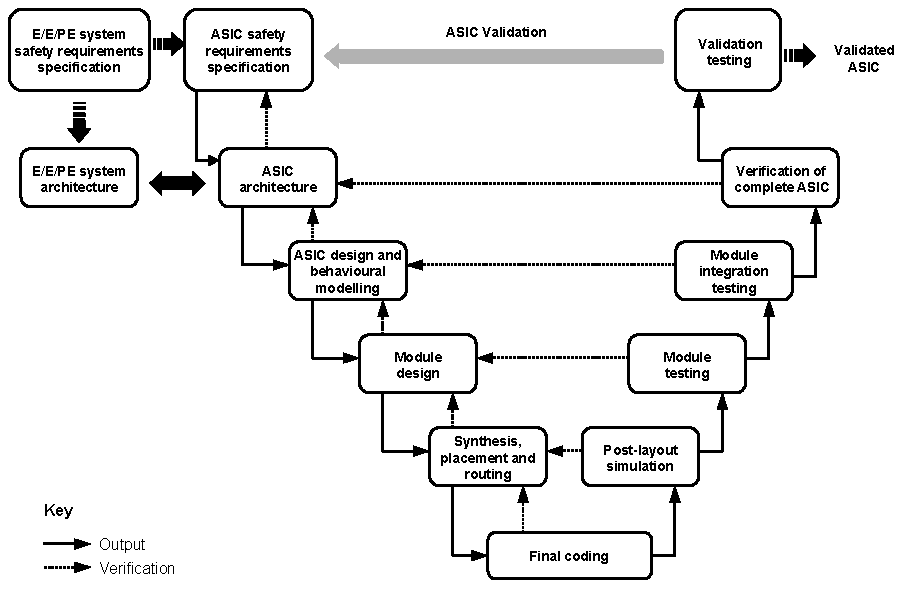
\includegraphics[width=0.8\textwidth]{images/Vmodel.pdf}
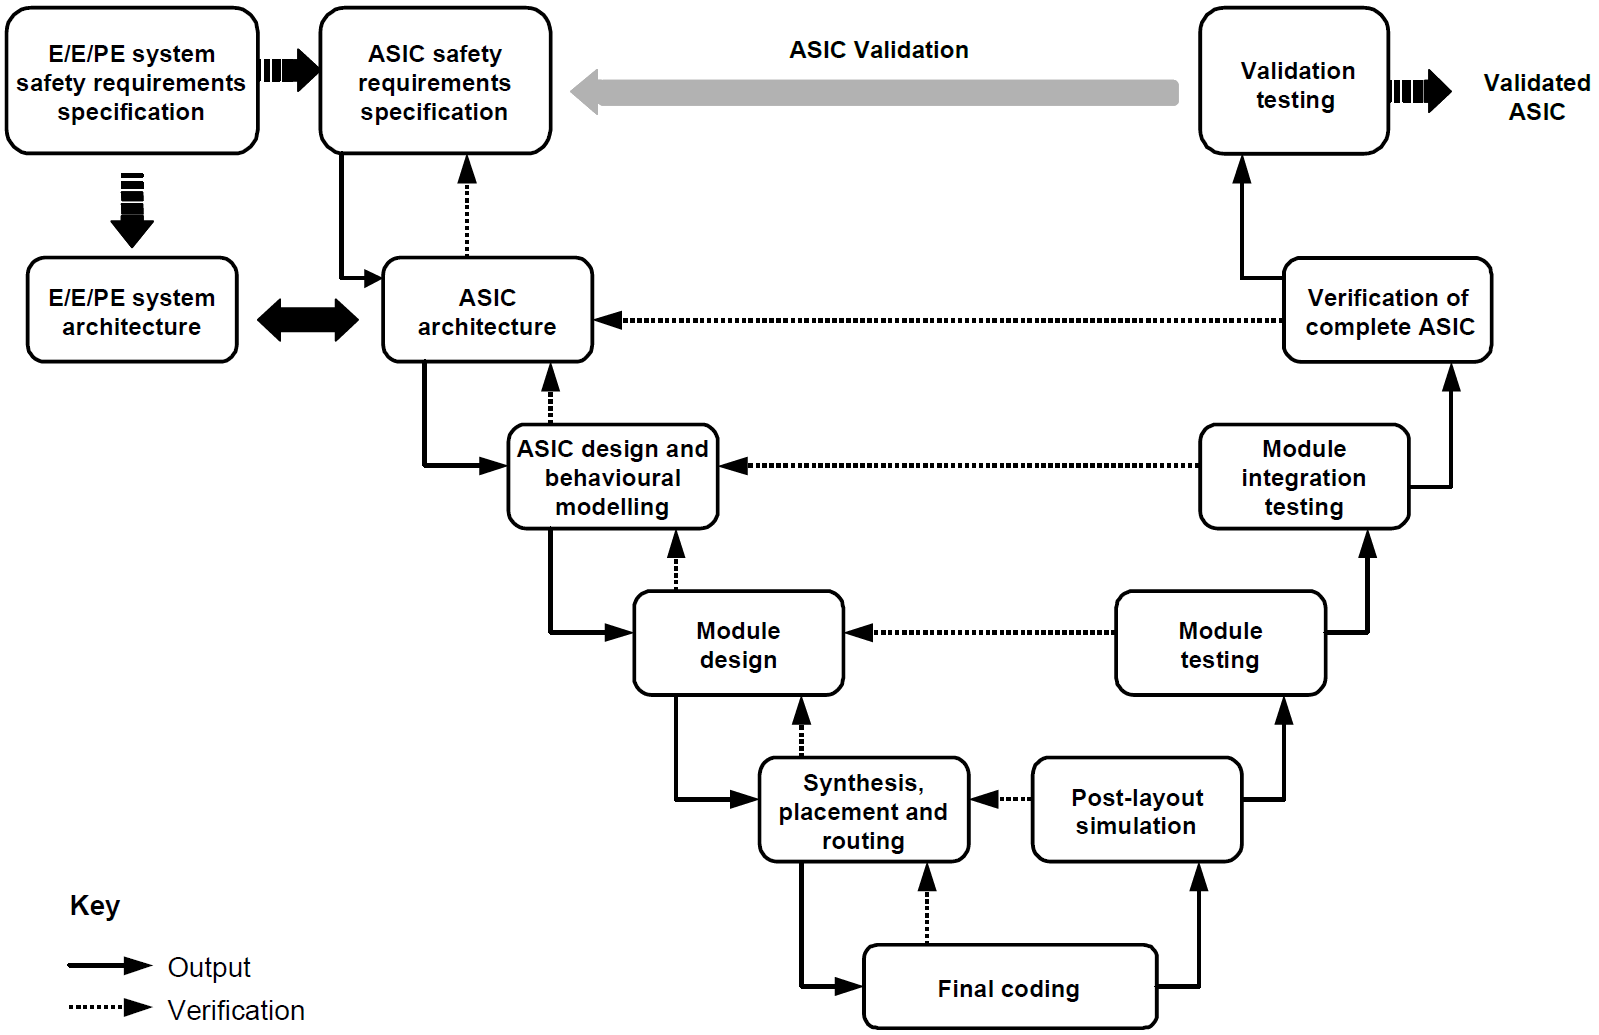
\includegraphics[width=\textwidth]{images/V-model.PNG}
\caption{The V-model for ASIC development adopted for design and verification in this project\cite{IEC61508}}
\label{V-model}
\end{figure}

Adoption of the V-model, see Figure \ref{V-model}, for ASIC and FPGA designs is recommended by Lattice for safety-related development\cite{LatticeSafety} as well as in the safety standards \cite{Borcsok, IEC61508, HayekSRAM, HayekSafety, Bernardeschi}. The model focuses on the verification and validation of the design at each design phase\cite{Borcsok}. For each design phase, there is a corresponding verification activity\cite{Ceesay-Seitz,Borcsok}. It incorporates methodologies from software development into the ASIC design process\cite{HayekSRAM}. As well as acting as an overall model for project development, the V-model can be traversed for subsystems and modules within the design\cite{Ceesay-Seitz}. HDLs support the adoption of the V-model as they allow for the behaviour and performance to be verified at each development phase of the project\cite{Dubey}.

\subsection{VHDL Verification Methodologies}

In order to tackle the increasing verification effort of FPGA designs, verification methodologies have emerged\cite{Foster}. There are a number of verification methodologies applicable to FPGAs and VHDL development. Verification is a large component of the design life-cycle. % find sources for this
Tallaksen finds that verification accounts for 50\% of the development effort for FPGA-based system\cite{Tallaksen}. It is a crucial activity which produces a valuable resource: automated and comprehensive test-suites provide a safety-blanket to ensure that any errors in the design are flagged\cite{janzen}.
%\subsection{Universal VHDL Verification Methodology}
One methodology, which is rapidly growing in popularity, is the Universal VHDL Verification Methodology (UVVM)\cite{Foster, Tallaksen}. The UVVM framework claims to provide overview, modifiability, debuggability and reusability to unstructured test-benches\cite{Tallaksen}.
%\subsection{Open Source VHDL Verification Methodology}
OSVVM (Open Source VHDL Verification Methodology) and UVVM have seen a considerable adoption for verification in FPGA-based design projects; in 2018 this was found to be 15\% and 10\% respectively\cite{Foster,Tallaksen}.

\section{Literature Review Conclusion} % should this be labelled? 

% safety standards being followed
FPGAs have seen considerable adoption in safety-critical and motor control. The relevant safety standards for the project are the IEC 61508 standards related to electronics development in safety-critical applications. Although there is no direct mention of FPGAs in this particular standard, FPGAs can be considered as ASICs throughout the development phases. 
The primary advantages of using FPGAs for safety-critical systems is having the ability to accurately model and verify timings and behaviour.
% increased verification effort -> verification methodologies -> functional safety now achievable
Advancements in FPGA technology have resulted in more complicated designs with multiple interfaces. This has introduced a significant verification requirement meaning that classic test-benches are no longer viable for complete verification. Verification methodologies, which have recently emerged, allow for the functional safety of FPGA systems to be achieved and proven. FPGAs also provide an elegant solution to component obsolescence, for which safety-critical systems are particularly vulnerable. 

% lack of coverage means the adoption of asic and software standards?
%Despite the increased adoption of FPGAs in safety-critical systems, there is a lack of FPGA-specific safety standards. This has resulted in the adoption of general standards and standards for related technologies which often fail to cover considerations specific to FPGAs.


% adoption of the v-model throughout the project 
The V-model, which is recommended for the standards, will be followed throughout the development of this project. It also forms the structure of this report. The following two sections traverse the V-model, discussing the high-level processes within the project. The design section, Section \ref{design}, discusses each of the activities on the left side of the V-model. In the verification section, Section \ref{verification}, the corresponding verification activities for each of the design phases are described. These are the activities on the right side of the V-model.



